\documentclass[tikz,border=7pt]{standalone}
\begin{document}
  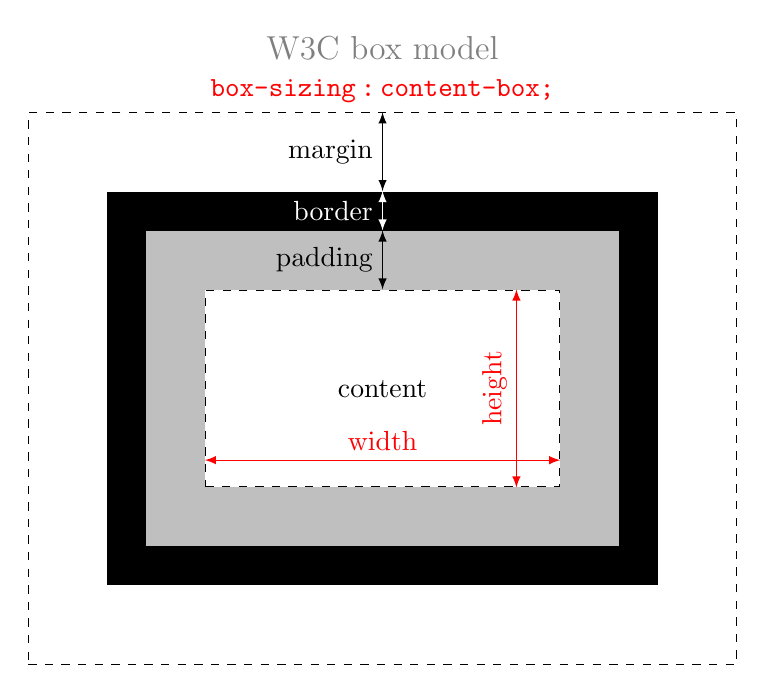
\begin{tikzpicture}[>=latex]
    \coordinate (O);
    % margin
    \node[draw, dashed, minimum width=9cm, minimum height=7cm] (M) {};
    % border
    \node[fill=black, dashed, minimum width=7cm, minimum height=5cm] (B) {};
    % padding
    \node[fill=lightgray, dashed, minimum width=6cm, minimum height=4cm] (P) {};
    % content
    \node[fill=white, draw, dashed, minimum width=4.5cm, minimum height=2.5cm] (C) {};
    \node at (C.center) {content};
    % width and height positions
    \coordinate (W) at (0,-.91);
    \coordinate (H) at (1.7,0);

    % arrows
    \draw[<->] (M.north) -- node[left] {margin} (B.north);
    \draw[<->, white] (B.north) -- node[left] {border} (P.north);
    \draw[<->] (P.north) -- node[left] {padding} (C.north);
    \draw[<->,red] (C.south-|H) -- node[sloped,above] {height} (C.north-|H);
    \draw[<->,red] (C.west|-W) -- node[above] {width} (C.east|-W);

    % title
    \path (M.north) node[red, above, font=\ttfamily] (CSS) {box-sizing\,:\,content-box;};
    \path (CSS.north) node[above, gray, font=\large] {W3C box model};
  \end{tikzpicture}
\end{document}
